\chapter{Introducción\label{01intro}}

% En los últimos años, el volumen de datos consumidos por muchas organizaciones ha explotado, debido a la explosión de la web, La llamada Web 2.0. 
% [Añadir fuente$^1$] En 15 de los 17 sectores económicos de los Estados Unidos, las empresas que tienen más de 1000 empleados, almacenan en promedio 
% más de 235 terabytes de datos que es más que el volumen de la biblioteca de datos del Congreso de los Estados Unidos. 

% Debido a la necesidad de escala y/o procesamiento, este volumen de datos ha aumentado y el mundo de las bases de datos creó una nueva técnica de 
% administración de datos con un modelo de gestión de datos novedoso llamado NoSQL (que significa ``no solo SQL''). Existe una amplia gama de soluciones 
% NoSQL y, en particular, más de 225.

% Tanto la investigación como la industria está utilizando estos sistemas de almacenamiento de datos a un ritmo muy rápido. En ambas áreas, los datos de 
% prueba son esenciales para las pruebas de rendimiento, de seguridad y las pruebas funcionales. 

% Los avances de la comunidad de investigación se usan ampliamente en una gran variedad de dominios de la informática como son privacidad, salud, reconocimiento 
% de patrones, minería de datos, etc. [Añadir fuente$^2$]

% En la actualidad desafortunadamente hay una escasez de disponibilidad de datos reales debido a que muchas organizaciones no están dispuestas a compartir sus 
% datos con terceros por garantizar la privacidad, el coste de la transferencia de los datos y la falta de disponibilidad de una cantidad enorme de datos. [Añadir fuente$^3$]
% Por lo tanto, el desarrollo y las pruebas de análisis de software son dependientes de los datos sintéticos que garantizan resultados lo más cercanos a la realidad posible.

A finales de la primera década de este siglo, las bases de datos NoSQL emergieron para paliar las limitaciones de los sistemas relacionales en el manejo de datos de las aplicaciones modernas surgidas con los avances tecnológicos como la Web 2.0, redes sociales, smartphones e IoT. Entre las nuevas características de las aplicaciones se encontraban la flexibilidad de soportar cambios frecuentes en los datos, datos que pueden ser muy complejos, la escalabilidad en el manejo de mayores volúmenes de datos ( "big data") y la disponibilidad continua.

En realidad, bajo el término NoSQL (no sólo SQL) se agrupan más de dos centenares de sistemas de bases datos que conforman a cuatro principales modelos de datos: documento, columnares, clave-valor, y grafos. Estos modelos tienen diferentes características incluso sistemas del mismo modelo. Sin embargo, hay algunos características que son comunes como (i)  que la mayoría de ellos están destinados a registrar datos semi-estructurados en los que el esquema es implícito por lo que no es necesaria la definición de un esquema antes de guardar datos (schemaless o schema-on-read), lo cual facilita la flexibilidad para aplicar cambios, (ii) lenguajes de consultas propios en vez de SQL, y transacciones no basadas en el teorema ACID, y (iii) proveen de escalabilidad horizontal.



\section{Motivación\label{01intro_motivacion}}

% En la actualidad el número de Sistemas Gestores de Bases de Datos (de aquí en adelante SGDB) ha aumentado en gran medida, sobre todo en el campo de las bases 
% de datos NoSQL (según \href{http://db-engines.com}{DB-Engines} de las 354 SGDB listadas 223 son NoSQL). Esto es provocado por la creación de nuevos softwares de almacenamiento 
% masivo y las facilidades que aportan los almacenamientos noSQL como la supresión de esquemas (schemaless) que hace muy fácil su utilización y versatilidad 
% en diversos campos.

Los primeros sistemas de bases de datos NoSQL aparecieron en grandes empresas de informática que necesitaban manejar las nuevas necesidades en su propia organización o en sus herramientas comerciales, como es el caso de Google con BigTable y Amazon con DynamoDB. Pronto, la comunidad científica prestó interés a los nuevos modelos y sistemas NoSQL y desde entonces un buen número de resultados de investigación se han publicado. Al igual que sucede con las bases de datos relacionales, el trabajo de investigación con datos NoSQL choca con la dificultad de disponer de datos reales para probar las soluciones ideadas para resolver los problemas identificados. Entre las dificultades encontradas, las empresas no pueden proporcionar datos por cuestiones de privacidad y los datasets disponibles no son apropiados para las pruebas que se desean realizar, entre otras. 

Por ello, la generación automática de datos NoSQL para validar y realizar testing sobre nuevas herramientas y enfoques es crucial, en muchas situaciones, grandes empresas como investigadores no pueden hacer uso de los datos reales debido un volumen insuficiente (estos casos pueden ser comparativas, evaluación de software, aprendizaje de inteligencias artificiales, machine learning, etc.). También es necesario que estos datos se puedan obtener en el formato deseado por los desarrolladores y que puedan adquirir la complejidad necesaria a la hora de evaluar posibles errores en el software..

La generación de datos sintéticos para sistemas NoSQL es más complicada que en el caso relacional ya que los diversos modelos de datos son más complejos. Las bases de datos relacionales definen bien sus tablas y no dejan escapar ninguna posibilidad de variación, estos esquemas permiten conocer qué tipos de datos contendrá la tabla en todo momento, si se repetirán, si pueden ser nulos, etc.

% Es por ello que los generadores de datos pensados para bases de datos relacionales no son suficientes para cubrir la necesidad de los no relacionales. En estos, al no haber esquemas, desconocemos la diversidad de los tipos de datos en una base de datos amplia. Un dato puede ser de dos tipos dependiendo de la situación, por ejemplo un precio puede venir dado en un número, o como una cadena donde se indica el símbolo de la moneda, puede incluso contener un objeto embebido el cual contenga el precio como número y el símbolo de la moneda como una cadena.

En cambio, en los sistemas NoSQL la ausencia de esquema provoca que los datos de una misma entidad pueden ser almacenados con diferentes estructuras, esto es, para cada tipo de entidad almacenada podrán existir una o más variaciones estructurales. Por ejemplo, en una entidad que representa productos, algunos campos podrían aparecer en todos los objetos almacenados pero otros no. Además, un campo podría aparecer con valores de distinto tipo, como el campo precio que podría estar almacenado en varias formas: en unos productos podría ser almacenado por un número, en otros como un string que incluye el valor numérico y un símbolo para el tipo de moneda, e incluso podría ser un dato embebido en el objeto producto que tuviese los campos precio y moneda. Por ello las generaciones de datos para nuevas bases de datos y SGDBs que las empresas deben testear para su desarrollo son necesarias incluso en mayor medida a las bases de datos relacionales tradicionales.

Las generaciones de datos son estrictamente necesarias para probar estructuras de bases de datos y SGDBs que las empresas deberán testar a la hora de comenzar un 
proyecto como fase de planificación para cubrir las necesidades a largo plazo.

% Por otra parte los generadores de datos no abundan en la actualidad, algunos más famosos como \href{https://mockaroo.com}{Mockaroo}, \href{https://generatedata.com}{Generatedata} u \href{https://onlinedatagenerator.com}{Online data generator} tienen soporte en la web, lo que proporciona facilidad para su uso y disponibilidad pero por contra tienen limitaciones en la generación debido a que la generación de datos se hace por parte de un servidor que debe ofrecer el servicio a un gran número de clientes. Otros programas como \href{https://datprof.com}{DATPROF} o  \href{https://sqlmanager.net}{SQL Manager} que sí son ilimitados y de instalación propia son comerciales, por lo que no son open-source ni gratuitos, suelen estar embebidos en programas más complejos de gestión de bases de datos además de no proporcionar las características antes mencionadas necesarias para gestores de bases de datos NoSQL.

En la actualidad hay disponibles algunos generadores gratuitos para la base de datos MongoDB como son \href{https://mockaroo.com}{Mockaroo} y \href{https://generatedata.com}{Generatedata}. El hecho de ser aplicaciones Web facilita su uso pero el servicio de generación es limitado en cuanto al tamaño y estructura de los datos generados. También hay herramientas comerciales como \href{https://datprof.com}{DATPROF} y \href{https://sqlmanager.net}{SQL Manager} que se integran en sistemas de bases de datos relacionales y aunque nos permitan crear generaciones sin límite de capacidad son exclusivamente para las propias bases de datos que gestionan que además son relacionales.

Todos estos generadores no ofrecen la posibilidad de establecer variación estructural para las entidades, ni tampoco establecer relaciones de composición y referencia entre entidades, además de las limitaciones antes mencionadas.

\section{Objetivos}

Como parte de la tesis de Alberto Hernández~\cite{deimosAlberto}, se ha desarrollado un enfoque de generación de datos destinado a solucionar los problemas de los citados anteriormente, limitación indefinida en la generación de datos, relaciones reales entre entidades, variabilidad de las estructura de los datos, entrada/salida de datos entre distintas bases de datos y/o ficheros con formatos definidos (CSV, JSON) y además deberá ser fácilmente usable y configurable a través de una generación pseudoaleatoria que el usuario podrá especificar para replicar la misma generación. La solución planteada está basada en la definición de un lenguaje para especificar las propiedades de los datos generados. Este lenguaje se denomina Deimos~\cite{deimosAlberto}. Con Deimos se podrán definir qué reglas contendrán los datos finales, su generación y los datos de entrada a través de ficheros o por consultas directas a bases de datos y por último la salida de estos datos.

El objetivo de este trabajo es extender la funcionalidad de Deimos con un generador de datos para testing de bases de datos NoSQL que genere entidades a partir de archivos Deimos, además deberá realizarlo de forma pseudoaleatoria, creando tipos de datos variables y utilizando toda la funcionalidad que Deimos provee. Este generador será de ámbito local y no una herramienta online para aportar una mayor potencia y una ilimitada capacidad de generación, contando con un gran abanico de opciones de entrada de datos de distintas fuentes para que el volumen de datos pueda ser lo más real posible.

\section{Metodología}

% Este trabajo se ha abordado utilizando el Proceso Unificado de Desarrollo Software~\cite{UML} o Proceso Unificado. Esta metodología de trabajo se establece en un marco de desarrollo software por casos de uso que se centra en la arquitectura y se basa en procesos iterativos e incrementales.

% El proceso Unificado realiza operaciones de forma iterativa e incremental compuesto de 4 fases: Inicio, elaboración, construcción y transición, que a su vez se dividen en varias etapas iterativas que dan como resultado un incremento del producto. Dentro de cada una de estas iteraciones se producen procedimientos en cascada que se recorren de forma clásica.

% \begin{figure}[h!]
% 	\centerline{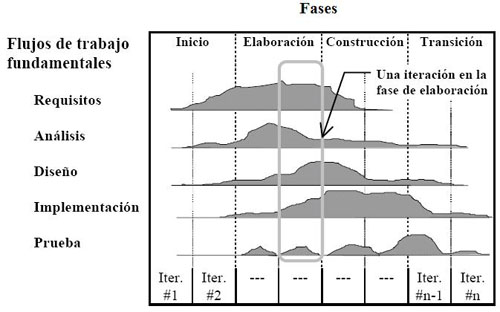
\includegraphics[width=1\textwidth]{uml_scheme.jpg}}
% 	\caption{Fases desarrollo en el Proceso unificado.}
% 	\label{figure:UML}
% \end{figure}

% En la figura podemos apreciar las fases y los flujos de trabajo que se realizan en cada una de ellas para diferenciar que mientras algunos flujos como los requisitos del desarrollo son realizados en las primeras etapas otros como los tests están presentes aunque no con igual importancia en prácticamente todas las fases del desarrollo.

% Es centrado en riesgos y dirigido por casos de uso, para ello se han realizado tests unitarios para ir superando cada una de las fases del desarrollo, buscando los puntos críticos del sistema, posibles errores y pruebas de rendimiento que garanticen una puesta en marcha óptima y sin errores.

Para la realización de este trabajo primero se realizó la planificación del mismo con los tutores, donde se comentó la finalidad del trabajo y como apoyaría la tesis de Alberto Hernández~\cite{deimosAlberto}. Una vez visto esto lo primero fue estudiar la semántica de Deimos, consultando dudas y aclarando conceptos de generación de datos para el funcionamiento del generador. Los tutores fueron proporcionando bibliografía acerca de las bases de datos NoSQL para comprender la necesidad de este generador y el lenguaje Deimos.

Por último, cabe destacar que se ha utilizado un repositorio github privado para compartir el trabajo con los tutores y Alberto, y el contacto con ellos se ha realizado a través de email y WhatsApp. En la primera etapa del trabajo se mantuvieron reuniones con los tutores y Alberto para resolver dudas y realizar un seguimiento del trabajo realizado. El trabajo se ha prolongado a lo largo de un año debido a que el estudiante compaginó su realización con un trabajo en la empresa de 9 horas diarias.

\section{Estructura del documento}

Este documento se organiza en los siguientes capítulos. El presente capítulo 1 ha
presentado el contexto, motivación, objetivos y la metodología seguida. El capítulo 2 presenta fundamentos de las bases de datos NoSQL y una Introducción al sistema de gestión de bases de datos NoSQL MongoDB, el capítulo 3 hace un recorrido por las soluciones vigentes que podemos encontrar a día de hoy para motivar la implementación de este trabajo, el capítulo 4 tratará los objetivos del trabajo, tecnologías a utilizar y el marco en el que se encuentra, el capítulo 5 trata de la implementación del generador, su uso, funcionalidad y cómo ha sido construido y por último el capítulo 8 recoge las conclusiones obtenibles del trabajo realizado, así como una serie de vías futuras con el propósito de ampliar y extender el trabajo realizado.

%%% Local variables:
%%% TeX-master: "memoria.tex"
%%% coding: utf-8
%%% ispell-local-dictionary: "spanish"
%%% TeX-parse-self: t
%%% TeX-auto-save: t
%%% fill-column: 75
%%% End:
